\documentclass{article}
\usepackage[utf8]{inputenc}

\usepackage{geometry}
\usepackage{bm}
\geometry{a4paper}
\usepackage{latexsym}
%\usepackage[dvips]{graphicx}
\usepackage{epsfig}
\usepackage{amsmath}
\usepackage{amsfonts}
\usepackage{amssymb}
\usepackage{eucal}
\usepackage{mathrsfs}
\usepackage{wasysym}
\usepackage{setspace}
\usepackage{float}
\usepackage{color}
\usepackage{rotating}
\usepackage{stmaryrd}
\usepackage{lineno}

\numberwithin{equation}{section}
\frenchspacing
%%
\usepackage{amsthm}


%%%%INSERITI ADESSO%%%%
\usepackage{amsmath}
\usepackage{amsfonts}
\usepackage{amssymb}
\usepackage{amsthm}
\usepackage{mathrsfs}
\usepackage{eucal}  
\theoremstyle{definition}
\usepackage{accents}
\usepackage{array}
\usepackage{cases}
\usepackage{graphicx}
\usepackage{booktabs}
\usepackage{caption}
\usepackage{cancel}
\usepackage{bbm}
\usepackage{subfig}
\usepackage{enumitem}
\usepackage{movie15}
 \usepackage{algorithm}
\usepackage{algpseudocode}
\usepackage{tabularx}
\usepackage{longtable}
 
% Font Management
\usepackage[T1]{fontenc}       % 8 bit font encoding: includes all accents
\usepackage{bm}                % alternative to \bs provided by package amsmath
\usepackage{bbm}               % alternative to \mathbb;  usage: \mathbbm{}
%\usepackage[mathscr]{eucal}    % alternative to \mathcal; usage: \mathcal{}
\usepackage{color}             % for text in colour
\usepackage{verbatim}          % environment for commenting out blocks of text
%\usepackage{exscale}           % needed to scale cmdx fonts
%\usepackage{ae,aecompl}        % see http://www.ctan.org/tex-archive/fonts/ae
%%%%%%%%%%%%%%%%%%



\theoremstyle{plain}
\newtheorem{thm}{Teorema}[section]
\newtheorem{lem}[thm]{Lemma}
\newtheorem{prop}[thm]{Proposizione}
\newtheorem*{cor}{Corollario}

\theoremstyle{definition}
\newtheorem{defn}{Definizione}[section]
\newtheorem{conj}{Congettura}[section]
\newtheorem{exmp}{Esempio}[section]

\theoremstyle{remark}
\newtheorem*{rem}{Osservazione}
\newtheorem*{note}{Nota}

\DeclareMathOperator*{\argmin}{argmin}
\DeclareMathOperator*{\argmax}{argmax}

\newcommand{\dom}{\mathrm{dom}}
\newcommand{\im}{\mathrm{im}}
\newcommand{\sign}{\mathrm{sign}}
\newcommand{\abs}{\mathrm{abs}}
\newcommand{\e}{\mathrm{exp}}

\setlength{\textwidth}{15 cm}
\setlength{\textheight}{23.5 cm}



%%%%%%%%%%%%%%%%%%%%%%%%%%%%%%%%%%%%%%%%%%%%%%%%%%%

\usepackage[utf8]{inputenc}
\usepackage[T1]{fontenc}
\usepackage{lmodern}

\usepackage{hyperref}
\hypersetup{%
    pdfpagemode={UseOutlines},
    bookmarksopen,
    pdfstartview={FitH},
    colorlinks,
    linkcolor={blue},
    citecolor={blue},
    urlcolor={blue}
  }

%%%%%%% use PDFLATEX 

\usepackage{lipsum} %to insert random text

\usepackage{geometry} %for the margins
\newcommand\fillin[1][4cm]{\makebox[#1]{\dotfill}} %for the dotted line in the frontispiace

\usepackage{dcolumn}
\newcolumntype{d}{D{.}{.}{-1} } %to vetical align numbers in tables, along the decimal dot

\usepackage{amsmath}



%%%%%%% Local definitions
\newtheorem{osservazione}{Osservazione}% Standard LaTeX
\newtheorem{observation}{Observation}% Standard LaTeX

\newcommand{\BR}{\mathscr{B}_{\mathrm{R}}}
\newcommand{\T}[2]{T_{#2}#1}
\newcommand{\cT}[2]{T_{#2}^{*}#1}
\newcommand{\pder}[2]{\frac{\partial #1}{\partial #2}}

				 
%%%%%%%%%%%%%%%%%%%%%%%%%%%%%%%%%%%%%%%%%%%%%%%%%
%
% Inserito il codice Matlab
%
\usepackage{listings}
\usepackage{hyperref}
\usepackage{xcolor}

\definecolor{codegreen}{rgb}{0,0.6,0}
\definecolor{codegray}{rgb}{0.5,0.5,0.5}
\definecolor{codepurple}{rgb}{0.58,0,0.82}
\definecolor{backcolour}{rgb}{0.95,0.95,0.92}

\lstdefinestyle{mystyle}{
    backgroundcolor=\color{backcolour},   
    commentstyle=\color{codegreen},
    keywordstyle=\color{magenta},
    numberstyle=\tiny\color{codegray},
    stringstyle=\color{codepurple},
    basicstyle=\ttfamily\footnotesize,
    breakatwhitespace=false,         
    breaklines=true,                 
    captionpos=b,                    
    keepspaces=true,                 
    numbers=left,                    
    numbersep=4pt,                  
    showspaces=false,                
    showstringspaces=false,
    showtabs=false,                  
    tabsize=2
}

\lstset{style=mystyle}


\title{Apprendimento Statistico}
\author{Nenna Giulio}
\date{Data Analysis applied to a Marketing Dataset}
\begin{document}
\maketitle
\section{Introduction} 
The main goal of this report is to apply different machine learning tecniques to a \href{http://archive.ics.uci.edu/ml/datasets/Bank+Marketing}{dataset} that can be found on the \href{http://archive.ics.uci.edu/ml/index.php}{UCI Machine Learning Repository}. The data is related with direct marketing campaigns (phone calls) of a Portuguese banking institution. Each entry represents a phone call to a client of whom several features are provided. \\
\\
The responce variable is binary (yes or no) and indicates whether a phone call successfully convinced the client to purchase a financial product the bank is tryng to sell (bank term deposit). Among the 20 provided features, 11 are categorical and the remaining are numerical. An extensive description of each feature will now follow.

\subsection{Attribute information}
Table \ref{table_attributes} provides an extensive overview about each attribute featured in the dataset.
\\
\\
Important notes about some of the attributes are the following:
\begin{description}
  \item[$\bullet$] Attributes from \texttt{Contact} to \texttt{duration} are related to the last contact of the current campaign
  \item[$\bullet$ ] The attribute \texttt{duration} affers to the call duration and it's not known until the call is completed. It highly affects the prediction (e.g. if \texttt{duration=0} then the outcome will always be \textit{not successful}), hence it will be deleted since the model is ment to be deployed with real world data.  
\end{description}

\begin{table}[H]
  \begin{tabularx}{\textwidth}{|X|X|X|X|}
    
    \hline
   Name & Description & Type & Possible values \\
   \hline
   \hline
   Age&Age of each client&numeric&- \\
   \hline
   Job& Type of job& categorical& Admn, blue-collar, entrepreneur...\\
   \hline
   Marital& Marital Status& categorical & Divorced, married, single, unknown\\
   \hline
   Education& level of education& categorical& basic.4y, basic.6y, basic.9y, high-school,...\\
   \hline
   Default&whether a client has credit in default & Categorical & Yes, No, Unknown\\
   \hline
   Housing& whether a client has an housing loan& Categorical & Yes, No, Unknown\\
   \hline
   Loan& whether a client has a personal loan& Categorical & Yes, No, Unknown\\
   \hline
   Contact& contact communication type& Categorical& cellular, telephone\\
   \hline
   Month& last contact month of the yeah& Categorical & jan, feb, mar...\\
   \hline
   Day of the week& last contact day of the week& Categorical & mon, tue, ...\\
   \hline
   Duration& Last contact duration in seconds (see notes)& Numeric&-\\
   \hline
   Campaign& number of contacts performed during this campaign for that client& Numeric& - \\
   \hline
   pdays& number of days that passed by after the client was last contacted from a previous campaign& numeric&-\\
   \hline
   previous& number of contacts performed before this campaign for this client& numeric&-\\
   \hline
   poutcome& outcome of the previous marketing campaign& Categorical & Failure, nonexistent, success\\
   \hline
   emp.var.rate& employment variation rate - quarterly indicator & Numeric &- \\
   \hline
   cons.price.idx& consumer price index - monthly indicator & Numeric & - \\
   \hline
   cons.conf.idx& consumer conficence index - monthly indicator & Numeric & - \\
   \hline
   euribor3m & euribor 3 month rate - daily indicator & Numeric & -\\
   \hline
   nr.employed& Number of employees - quarterly indicator & Numeric & - \\
   \hline
   \textbf{Responce variable: } \texttt{y} & Has the client subscribed to a term deposit & Binary & Yes, No\\
   \hline
\end{tabularx}
\caption{Extensive description for each attribute in the dataframe}
\label{table_attributes}
\end{table}

\section{Data Exploration and Preprocessing}
We first import the dataset and encode each categorical feature using \textit{one-hot encoding}. This means that numerical features will be left unchanged while for each categorical feature the process is the following:
\begin{description}
    \item[1.] Determine all the distinct values of that feature (categories)
    \item[2.] For each category generate a new binary column
    \item[3.] Assign values to the binary columns according to categories featred in each line.   
\end{description}
\begin{center}
    \begin{tabular}{|c|}
        \hline
        feature \\
        \hline
        \hline
        category 1 \\
        \hline
        category 2 \\
        \hline
        category 3 \\
        \hline
        category 2 \\
        \hline
    \end{tabular}
    \quad
    \begin{tabular}{|c|c|c|}
        \hline
        category 1 & category 2 & category 3\\
        \hline
        \hline
        1 & 0 & 0 \\
        \hline
        0 & 1 & 0 \\
        \hline 
        0 & 0 & 1 \\
        \hline
        0 & 1 & 0 \\
        \hline
    \end{tabular}    
\end{center}
\begin{lstlisting}[language=Python, caption= Data encoding]
    import pandas as pd

    df = pd.read_csv('Data/bank/bank-additional-full.csv', sep=';')
    display(df.head())
    cat_col = df.dtypes=='O'
    df_enc = pd.get_dummies(df.loc[:, cat_col], prefix=df.columns[cat_col])
    df_enc = df_enc.join(df.loc[:, np.logical_not(cat_col)])

    df_enc = df_enc.drop('y_no', axis=1) #deleting column since attribute "y" is binary
    df_enc = df_enc.drop('duration', axis = 1) #drop the duration column (see attribute information)

\end{lstlisting}

\subsection{Data Exploration}
In order to gain useful insights about some of the attributes featured in the dataset we can now perfom some \textit{data exploration}. This step of the analysis is qualitative by nature and consists in plotting graphs and distributions relative to each feature in the dataset.\\
\\
 There are 11 categorical features and the remaining are numerical. Categorical data will be explored by means of \textit{pie charts} while numerical data will be explored by means of a \textit{scatterplot matrix}

\begin{figure}[H]
    \centering
    \subfloat[1][Pieplot relative to \texttt{job}]{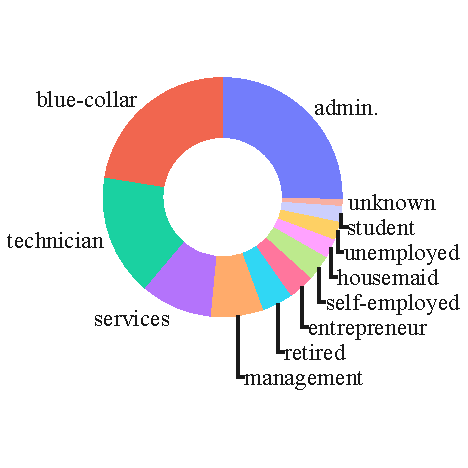
\includegraphics[scale = 0.8]{pictures/pieplot0_job.pdf}}
    \qquad
    \qquad
    \subfloat[2][Pieplot relative to \texttt{marital}]{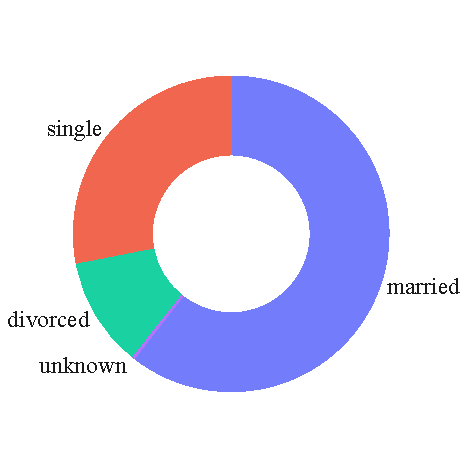
\includegraphics[scale = 0.8]{pictures/pieplot1_marital.pdf}}
\end{figure}

\begin{figure}[H]
    \centering
    \subfloat[1][Pieplot relative to \texttt{education}]{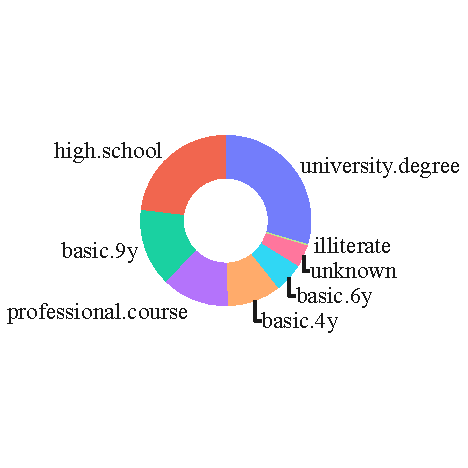
\includegraphics[scale = 0.8]{pictures/pieplot2_education.pdf}}
    \qquad
    \qquad
    \subfloat[2][Pieplot relative to \texttt{default}]{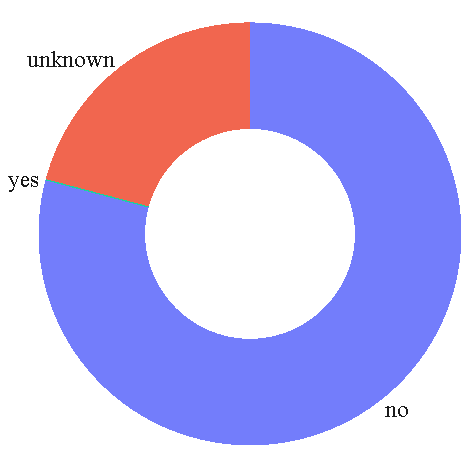
\includegraphics[scale = 0.8]{pictures/pieplot3_default.pdf}}
\end{figure}

\begin{figure}[H]
    \centering
    \subfloat[1][Pieplot relative to \texttt{housing}]{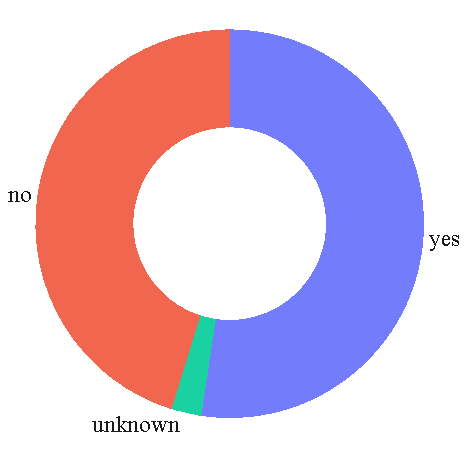
\includegraphics[scale = 0.8]{pictures/pieplot4_housing.pdf}}
    \qquad
    \qquad
    \subfloat[2][Pieplot relative to \texttt{loan}]{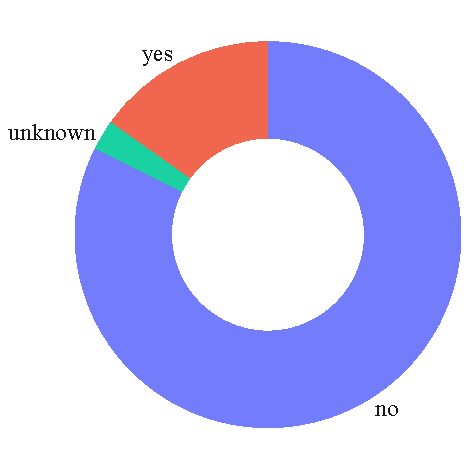
\includegraphics[scale = 0.8]{pictures/pieplot5_loan.pdf}}
\end{figure}

\begin{figure}[H]
    \centering
    \subfloat[1][Pieplot relative to \texttt{contact}]{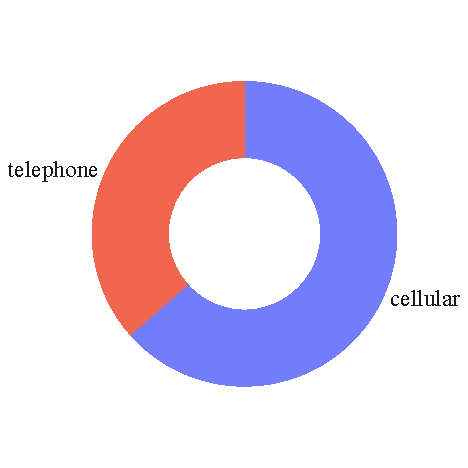
\includegraphics[scale = 0.8]{pictures/pieplot6_contact.pdf}}
    \qquad
    \qquad
    \subfloat[2][Pieplot relative to \texttt{month}]{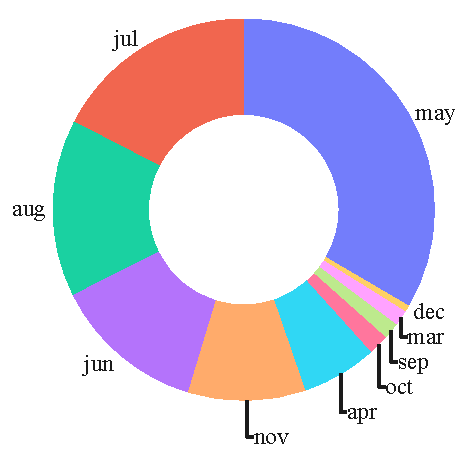
\includegraphics[scale = 0.8]{pictures/pieplot7_month.pdf}}
\end{figure}
\begin{figure}[H]
    \centering
    \subfloat[1][Pieplot relative to \texttt{day\_of\_the\_week}]{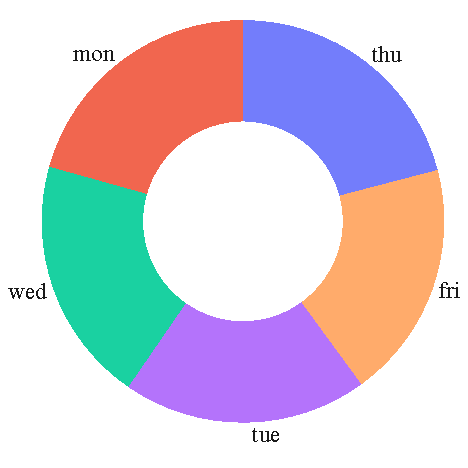
\includegraphics[scale = 0.8]{pictures/pieplot8_day_of_week.pdf}}
    \qquad
    \qquad
    \subfloat[2][Pieplot relative to \texttt{poutcome}]{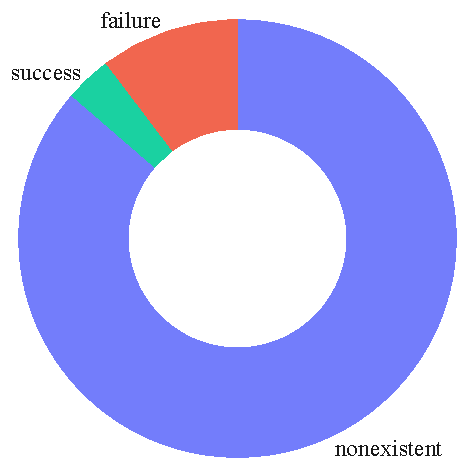
\includegraphics[scale = 0.8]{pictures/pieplot9_poutcome.pdf}}
\end{figure}

\begin{figure}[H]
    \centering
    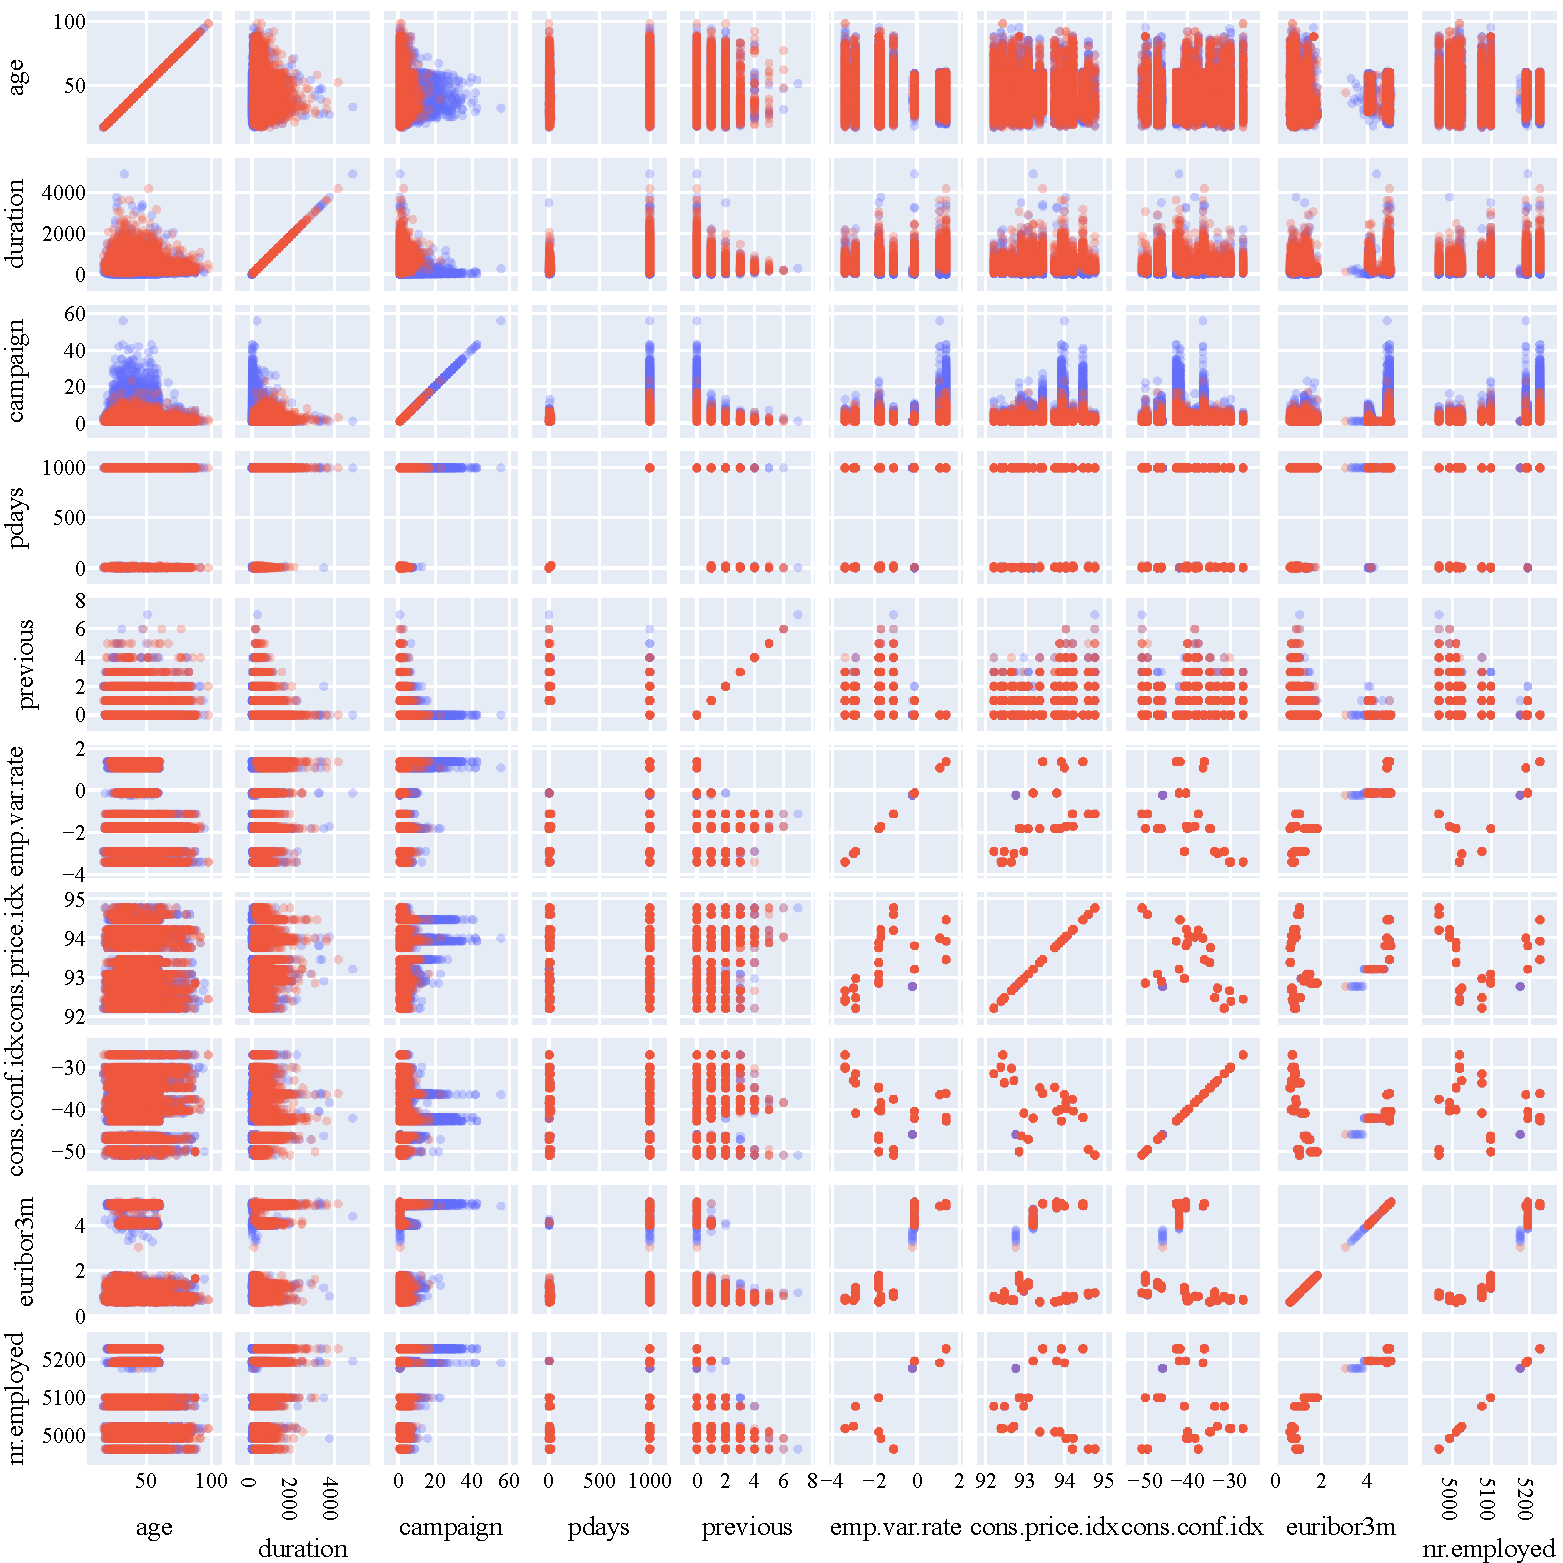
\includegraphics[scale=0.55]{pictures/scatterplot.pdf}
    \caption{Scatterplot matrix of numerical features }
\end{figure}
From the scatterplot we don't see any particular correlation between numerical features. Yet, as for the coloring of the data, one can notice that the attribute \texttt{campaign} discriminates pretty well the outcome. As a matter of fact people that recieved a lot of calls from the call center never buy the product that the bank is trying to sell. This information alone could be of some value for reducing cost and better targeting calls.

\subsection{Dataset splitting} \label{dataset_splitting}
After exploring data, the first thing to do is to perform a split of our dataset into training and test set.
\begin{lstlisting}[language=Python, caption= Data splitting]
    df_train, df_test = train_test_split(df_enc, test_size=0.1, random_state=42)
\end{lstlisting}
As it is the case with some binary classification datasets, our data is heavly biased towards one class of outcome. In our case the most common outcome for each call is, reasonably, unsuccesful call: meaning that the client that has been called have \textbf{not} purchased the product that the bank is trying to sell. In order to quantify the class unbalance we can use a simple pie chart:

\begin{figure}[H]
    \centering
    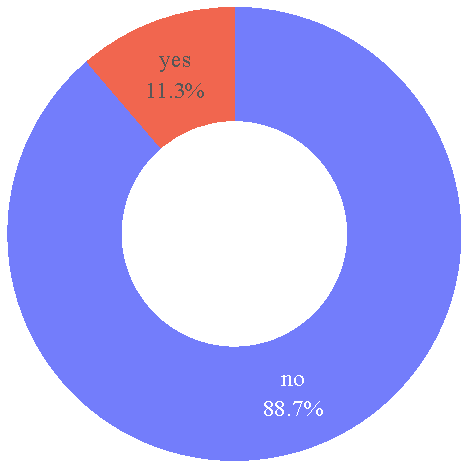
\includegraphics[scale=0.8]{pictures/pieplot_unbalance.pdf}

    \caption{Responce variable class unbalance}
\end{figure}

As we can see $\sim 90\%$ of our data is biased towards the majority class (no). If we tried to feed the data as it is to any classification model the resulting classifier would seem to be "accurate" even if it really isn't.\\
\\
As a simple example we could think of a classifier that classifies every data entry as "unsuccesful call" no matter of the features. This naive classifier, tested with our heavily biased data, would result to have $\sim 90\%$ accuracy, the same percentage of the majority class with respect to the whole dataset.\\
\\
Various techniques can be used in order to solve this problem, among them there are \textbf{Oversampling} and \textbf{Undersampling}. 

\begin{figure}[H]
    \centering
    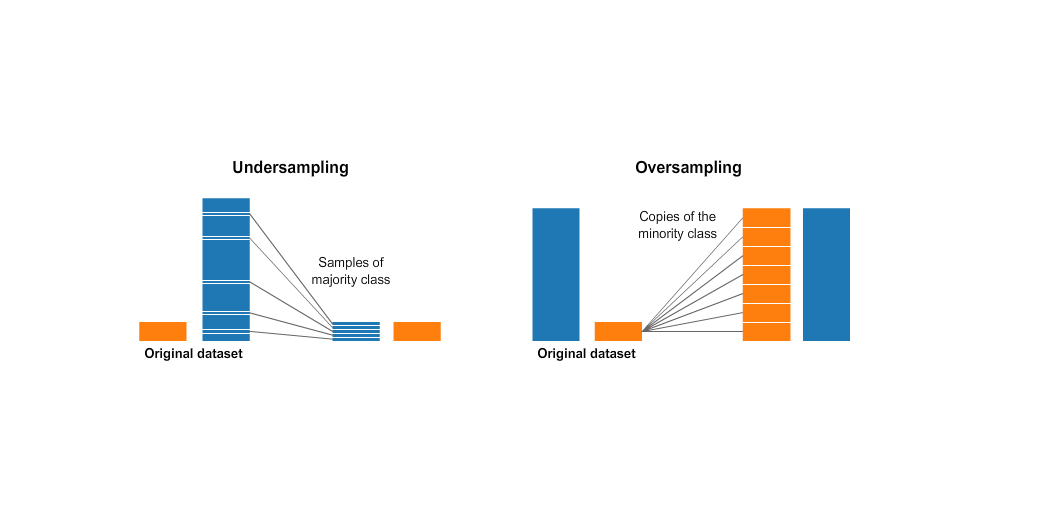
\includegraphics[scale=0.4]{pictures/undersampling-oversampling.png}

    \caption*{Visual exapmple of Oversampling and Undersampling}
\end{figure}
As the name suggests, oversampling takes place when the minority class is used to generate new bootstrapped data to balance classess. On the other hand, undersampling consists in randomly sampling from the majority class enough samples such that the two classes are balanced. In our case, since we have enough data, we can opt for undersampling in order to balance classes.

\begin{lstlisting}[language=Python, caption= Data rebalancing]
response = df_train['y_yes']
feature_matrix = df_train.loc[:, df_train.columns!='y_yes']

#rebalancing classes (y_yes=1 is the minority class)--------
ratio = df_train['y_yes'].sum()/df_train['y_yes'].size
print("Original training dataset has", df_train.index.size, "Observations. \n", "Among them", response.sum(), "are positive and", response.size-response.sum(), "are negative \n Performing dataset rebalancing by undersampling... \n\n" )
df_train_false = df_train.loc[response==0, :]
df_train_false_resampled = df_train_false.sample(frac=ratio)

df_train_true = df_train.loc[response==1,:]

df_train = pd.concat([df_train_true, df_train_false_resampled])
ratio = df_train['y_yes'].sum()/df_train['y_yes'].size

response = df_train['y_yes']
feature_matrix = df_train.loc[:, df_enc.columns!='y_yes']

print("Training Dataset rebalancing performed. Dataset has now", df_train.index.size, "Observations. \n", "Among them", response.sum(), "are positive and", response.size-response.sum(), "are negative \n\n" )

X_train = df_train.loc[:, df_train.columns!='y_yes']
X_test = df_test.loc[:, df_test.columns!='y_yes']
y_train = df_train['y_yes']
y_test = df_test['y_yes']

\end{lstlisting}
One can notice that only the training tast was subject to the rebalancing process. This is because real-world data will not be balanced and rebalancing test data would cause the same problems concearning test accuracy.

\subsection{Scaling the dataset}

The encoded dataset is characterized by features with very different scale/range  of values. In this case, if we apply PCA or any kind of training model on this data, some important features can be "covered" by other feature just for the unit measure disparity. This is why is a good practice to \textbf{rescale} the data. The most used scalers used are the \textbf{Min-max Scaler} and \textbf{Standard Scaler}.\\
\\
The \textbf{Min-Max Scaler} trasnforms the data such that the values of each column are distributed between a minimum value $m$ and a maximum value $M$. Let $X \in \mathbb{R}^{n \times p}$ be our feature matrix, with $X=[x_1, x_2, \dots, x_p]$. Let $X' \in \mathbb{R}^{n \times p}$ be our scaled matrix with $X'=[x'_1, x'_2, \dots, x'_p]$. If $M_i = \max\{x_i\}$, $m_i = \min\{x_i\}$, $i \in \{1,  \dots,  p\}$ then
\begin{align}
    x'_i = \frac{x_i - m_i}{M_i-m_i}, && i \in \{1,  \dots,  p\}    
\end{align}
where all operations are intended to be element-wise. \\
\\
On the other hand the \textbf{Standard-Scaler} makes the values of each feature in the data to have zero-mean and unit-variance. In particular: 
\begin{align}
    x'_i = \frac{x_i - \bar{x_i}}{s_i}, && i \in \{1,  \dots,  p\}    
\end{align}
where $\bar{x_i}$ is the \textit{sample mean} and $s_i$ is the \textit{sample variance} of the $i$-th column
\begin{lstlisting}[language=Python, caption= Data scaling]
#Performing scaling using min-max scaler
scaler_mm = MinMaxScaler()
scaler_mm.fit(X_train)

X_train_scaled_mm = scaler_mm.transform(X_train)
X_test_scaled_mm = scaler_mm.transform(X_test)

#Performing scaling using standard scaler
scaler_std = StandardScaler()
scaler_std.fit(X_train)

X_train_scaled_std = scaler_std.transform(X_train)
X_test_scaled_std = scaler_std.transform(X_test)
\end{lstlisting}
As it is the case with most steps in our analysis pipeline, scaling is \textit{fitted} on \textbf{training data}, meaning that all the values used for the scaling are computed on the training dataset. When performing a prediction, test data should also undergo the same rescaling process using however the values fitted with the training data. Not doing so would result in what in data analysis is called \textit{data leakage}, meaning that information about test data \textit{leaked} into the training process.

\subsection{Performing PCA on the dataset}
PCA stands for \textit{Principal Component Analysis} and is a technique used to reduce the dimensionality of the data (number of columns) while retaining as much information as possible.
\\
\\
Let \(X \in \mathbb{R}^{n \times p}\) be our feature matrix and let
\begin{equation}
    \Sigma = \frac{1}{N- 1} \bar{X}^T\bar{X} \in \mathbb{R}^{p \times p}
\end{equation}
Be the \textit{Covariance matrix} of \(X\), where \(\Bar{X}\) is the \textit{centered} data matrix i.e. \(\Bar{X} = [x_1 - \Bar{x_1}, \dots x_p - \Bar{x_p}]\) (all the columns of \(X\) are centered w.r.t. their sample mean). \\
Since the covariance matrix \(\Sigma\) of our centered data is a symmetric semi-definite positive matrix, we can compute its \textbf{eigendecomposition}:
\begin{equation}
    \Sigma = V \Lambda V^T
\end{equation}
with:
\begin{equation}
 V = [v_1, v_2, \dots, v_p] \in \mathbb{R}^{p \times p}, \qquad \Lambda = \begin{bmatrix}
    \lambda_1 & \dots & 0 \\
    \vdots & \ddots & 0 \\
    0 & \dots & \lambda_n
 \end{bmatrix}, \qquad \lambda_1 \geq \lambda_2 \geq \dots \geq 0.
\end{equation}
Then it can be shown that \textbf{the columns of \(V\) describe the directions of greater variance of data}, depending on the eigenvalues magnitude. This means that \(V\) is a new basis for \(\mathbb{R}^p\) and can be seen as a \textbf{rotation matrix}. Let \(x^{(i)}\in \mathbb{R}^p\), then \(y^{(i)} = V^T x^{(i)}\) is the same vector but represented with basis \(V\). By this token we could compute the rotation of each point in our original data \(X\) obtaining the matrix \(Y = \Bar{X}V\in \mathbb{R}^{n\times p}\). The resulting covariance matrix \(\Sigma_Y\) would be:
\begin{equation}
    \Sigma_Y = \frac{1}{N- 1} Y^T Y = V^T \Bar{X}^T \Bar{X} V = V^T \Sigma V = \Lambda
\end{equation}
This means that data written w.r.t. the new basis \(V\) has a diagonal covariance matrix \(\Lambda\) and the variance of \(Y\) w.r.t. the axis \(v_i\) is \(\lambda_i\). We call \(v_1, \dots , v_p\) \textbf{principal components} and \(\lambda_i\) is the \textbf{Explained variance} of the principal component \(v_i\). \\
\\
Since eigenvalues are computed in descreasing order, the first components of the data written in the basis \(V\) are the one with the most explained variance. Hence, truncating the rotated data matrix to the first \(k\) columns \((Y_k)\), causes a loss of explained variance that is quantified by the remaining \(\lambda_{k+ 1}\dots \lambda_p\) eigenvalues. The \textbf{percentage of explained variance} by the first \(k\) components is hence computed as:
\begin{equation}
     \texttt{ev\_ratio} = \frac{\sum \limits_{i= 1}^{k} \lambda_i}{\sum \limits_{i= 1}^{p} \lambda_i}. 
\end{equation}
\\
In figure \ref{fig_PCA} percentage of explained variance is plotted against the number of components, and we compare the performance of the \textit{min-max scaler} against the \textit{standard scaler} with respect to the explained variance.

\begin{lstlisting}[language=Python, caption= Data scaling]
#Performing pca using min max scaler

pca_mm = PCA()
pca_mm.fit(X_train_scaled_mm)
var_mm = pca_mm.explained_variance_ratio_

#performing pca using std scaler

pca_std = PCA()
pca_std.fit(X_train_scaled_std)
var_std = pca_std.explained_variance_ratio_

n_components=20

X_train_scaled_mm_pca = pca_mm.transform(X_train_scaled_mm)[:, :n_components]
X_test_scaled_mm_pca = pca_mm.transform(X_test_scaled_mm)[:, :n_components]
\end{lstlisting}
If the number of components to keep is fixed to \texttt{n\_components = 20} then, as we can see in figure \ref{fig_PCA}, data scaled with the min-max scaler retains more variance than the standard scaler. In particular with \(20\) principal components the percentage of explained variance computed on data scaled with the \textit{min-max scaler} is \(\sim 83\%\)
\begin{figure}[htb]
    \centering
    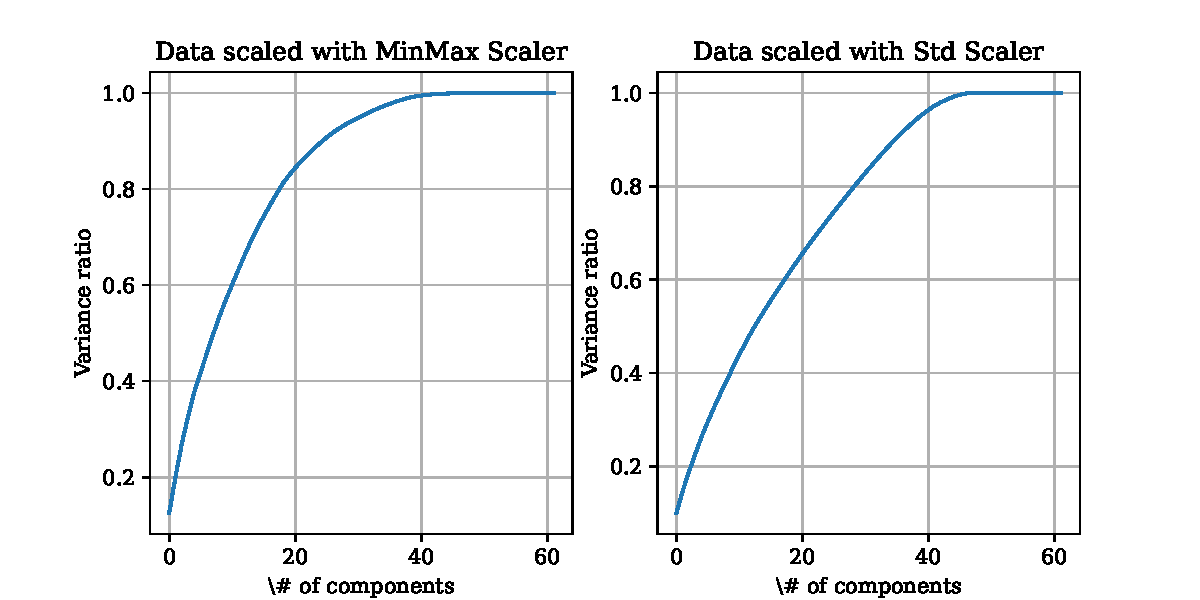
\includegraphics[scale=0.7]{pictures/variance_ratio_PCA.pdf}\
    \caption{Percentage of explained variance comparison between scalers}
    \label{fig_PCA}
\end{figure}




%\bibliographystyle{plain} % We choose the "plain" reference style
%\bibliography{refs} % Entries are in the refs.bib file


\end{document}